% ============================================================
%  Curriculum Vitae — Rocélio da Silva
%  v4 EN — English Version: larger type, looser leading, clearer hierarchy
% ============================================================
\documentclass[10pt,a4paper]{article}

\usepackage[utf8]{inputenc}
\usepackage[T1]{fontenc}
\usepackage[margin=0pt]{geometry}
\usepackage{array,tabularx}
\usepackage{enumitem}
\usepackage{titlesec}
\usepackage{hyperref}
\usepackage{xcolor}
\usepackage{graphicx}
\usepackage{tikz}
\usepackage{setspace}
\usepackage{parskip}
\usepackage{pagecolor}
\usepackage{amssymb}

\usetikzlibrary{calc}

\definecolor{sidebarBg}{HTML}{580000}
\definecolor{mainBg}{HTML}{7A0000}
\definecolor{cvgold}{HTML}{D4AF37}
\definecolor{cvgoldlt}{HTML}{EDD87A}
\definecolor{cvwhite}{HTML}{F7F2E8}
\definecolor{cvmuted}{HTML}{D8CCBA}

\pagecolor{mainBg}
\color{cvwhite}
\pagestyle{empty}
\setlength{\parindent}{0pt}
\setlength{\parskip}{2pt}

\hypersetup{colorlinks=true, urlcolor=cvgoldlt, linkcolor=cvgoldlt}

\let\tbf\textbf
\renewcommand{\textbf}[1]{{\bfseries\color{cvgold}#1}}

\newcommand{\sideSection}[1]{%
  \vspace{7pt}%
  {\bfseries\color{cvgold}\small\MakeUppercase{#1}}%
  \par\vspace{1pt}%
  {\color{cvgold}\rule{\linewidth}{0.55pt}}%
  \par\vspace{1pt}%
}

\newcommand{\mainSection}[1]{%
  \vspace{1pt}%
  {\bfseries\color{cvgold}\large\MakeUppercase{#1}}%
  \par\vspace{0pt}%
  {\color{cvgold}\rule{\linewidth}{0.9pt}}%
  \par\vspace{1pt}%
}

\newcommand{\expEntry}[3]{%
  {\bfseries\color{cvgold}\normalsize #1}\par\vspace{1pt}%
  {\color{cvmuted}\small #2 \hfill \textit{\color{cvgoldlt}#3}}\par\vspace{1pt}%
}

\setlist[itemize]{
  itemsep=1pt,
  topsep=1pt,
  leftmargin=1.3em,
  label={\color{cvgold}\small$\blacklozenge$}
}

\begin{document}

\noindent
\begin{tikzpicture}[remember picture, overlay]
  \fill[sidebarBg]
    (current page.north west)
    rectangle
    ([xshift=0.295\paperwidth] current page.south west);
  \draw[cvgold, line width=1.5pt]
    ([xshift=0.295\paperwidth] current page.north west)
    -- ([xshift=0.295\paperwidth] current page.south west);
\end{tikzpicture}

% ============================================================
%  LEFT SIDEBAR
% ============================================================
\noindent
\begin{minipage}[t]{0.283\paperwidth}
  \color{cvwhite}
  \setlength{\parskip}{3pt}
  \hspace*{10pt}%
  \begin{minipage}[t]{\dimexpr\linewidth-18pt}

    \vspace{5pt}
    \begin{center}
      \IfFileExists{photo.png}{%
        \begin{tikzpicture}
          \clip (0,0) circle (0.72in);
          \node[inner sep=0pt] at (0,0)
            {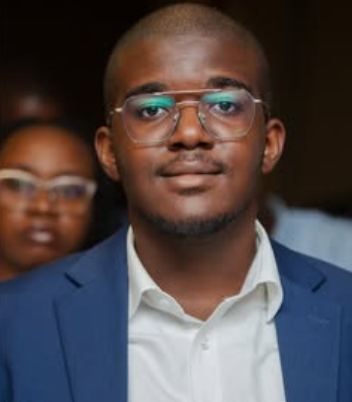
\includegraphics[width=1.44in,height=1.44in,keepaspectratio]{photo.png}};
          \draw[cvgold, line width=2pt] (0,0) circle (0.72in);
        \end{tikzpicture}%
      }{%
        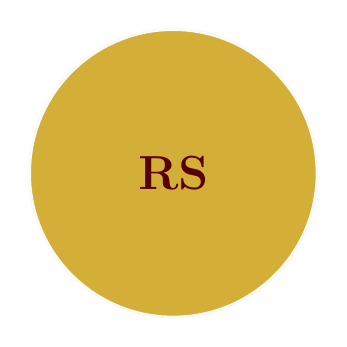
\begin{tikzpicture}
          \fill[cvgold] (0,0) circle (0.72in);
          \draw[cvwhite!40, line width=1.2pt] (0,0) circle (0.72in);
          \node[font=\bfseries\LARGE, text=sidebarBg] at (0,0) {RS};
        \end{tikzpicture}%
      }
      \par\vspace{2pt}
      {\large\bfseries\color{cvgold} Rocélio da Silva}\par\vspace{2pt}
      {\small\color{cvmuted} Offshore \& Upstream Engineering}\par\vspace{2pt}
      {\color{cvgold}\rule{0.70\linewidth}{0.5pt}}
    \end{center}

    \sideSection{Contact}
    {\small
      \textbf{Tel\,} \color{cvwhite}+244 924 010 222\par\vspace{2pt}
      \textbf{Email\,} \href{mailto:rocelioinc@gmail.com}{\color{cvgoldlt}rocelioinc@gmail.com}\par\vspace{2pt}
      \textbf{Local\,} \color{cvwhite}Benfica, Luanda\par
    }

    \sideSection{Education}
    {\small
      \textbf{ISPTEC}\par
      \color{cvwhite}B.Sc. Eng.\ de Petróleos\par
      \textit{\color{cvgoldlt}2022 -- Present $\cdot$ 3rd Year}\par\vspace{2pt}
      \textbf{CEPI}\par
      \color{cvwhite}Secondary Diploma\par
      \textit{\color{cvgoldlt}2020 -- 2022}\par
    }

    \sideSection{Languages}
    {\small
      \begin{tabular}{@{}l@{\hspace{6pt}}r@{}}
        \textbf{Portuguese} & \color{cvwhite}Native \\[3pt]
        \textbf{English}    & \color{cvgoldlt}TOEFL 99 \\
      \end{tabular}
    }

    \sideSection{Technical Skills}
    {\small
      \begin{itemize}[leftmargin=1em]
        \item Python -- Pandas, Matplotlib
        \item Calc. Z-Factor (Pitzer, Papay)
        \item Seleccao de metodos EOR
        \item Reservatorios \& Pocos
        \item Fluidos de Perfuracao Offshore
        \item GIS basico $\cdot$ Blender 3-D
        \item C,\; HTML / CSS
      \end{itemize}
    }

    \sideSection{Leadership}
    {\small
      \begin{itemize}[leftmargin=1em]
        \item Membership Chairperson
        \item Gestao de eventos
        \item Comunicacao tecnica
        \item Trabalho em equipa
      \end{itemize}
    }

    \sideSection{Affiliations}
    {\small
      \textbf{SPE} -- Soc.\ of Petroleum Engineers\par
      \textit{\color{cvgoldlt}Student Member}\par\vspace{2pt}
      \textbf{MIT Global Classroom}\par
      \textit{\color{cvgoldlt}Participant, 2025}\par
    }

    \vspace{2pt}
    \begin{center}
      {\color{cvgold}\rule{0.55\linewidth}{0.4pt}}\par\vspace{2pt}
      {\color{cvgoldlt}\small\itshape References upon request}
    \end{center}

  \end{minipage}
\end{minipage}%
%
% ============================================================
%  RIGHT MAIN
% ============================================================
\hspace*{10pt}%
\begin{minipage}[t]{\dimexpr 0.705\paperwidth - 26pt}
  \color{cvwhite}
  \setlength{\parskip}{1pt}
  \setstretch{1.03}

  \vspace{5pt}

  
\begin{tikzpicture}
    \node[inner sep=0pt, anchor=west] (title) at (0,0)
      {\parbox{\linewidth}{%
        {\huge\bfseries\color{cvgold} ROCELIO DA SILVA}\\[2pt]
        {\normalsize\color{cvmuted}
          Offshore \& Upstream Engineering $\cdot$ SPE Member $\cdot$ Luanda, Angola}%
      }};
    \draw[cvgold, line width=0.7pt]
      ([yshift=-4pt] title.south west) -- ([yshift=-4pt] title.south east);
  \end{tikzpicture}

  \mainSection{Profile}
  \setstretch{1.05}
  Estudante do 3.o ano de Engenharia de Petroleos no ISPTEC com forte vocacao para
  operacoes \textbf{offshore} e desenvolvimento de software tecnico para a industria
  petrolífera. Lider da equipa ISPTEC no PetroChamp, Membership Chairperson do SPE
  Student Chapter e participante do MIT Global Classroom (2025). Desenvolve ferramentas
  Python para calculos de engenharia de reservatorios (factor Z, EOR). Fluente em
  Ingles (TOEFL 99) e comprometido com excelencia tecnica em mercados emergentes.
  \setstretch{1.05}

  \mainSection{Professional Experience}

  \expEntry{Membership Chairperson -- SPE Student Chapter}%
           {ISPTEC / Society of Petroleum Engineers}%
           {2026 -- Presente}
  \begin{itemize}
    \item Lidera recrutamento, engagement e retencao de membros.
    \item Coordena seminarios tecnicos e promove networking industria-academia.
  \end{itemize}

  \vspace{2pt}
  \expEntry{Secretary of Academic Affairs}%
           {AEISPTEC -- Associacao de Estudantes do ISPTEC}%
           {2022 -- 2025}
  \begin{itemize}
    \item Coordenou eventos academicos e actividades departamentais.
    \item Geriu comunicacoes e documentacao academica dos estudantes.
    \item Serviu de liaison entre a lideranca academica e o corpo estudantil.
  \end{itemize}

  \mainSection{Key Projects}

  \textbf{Community Solar Feasibility Study -- MIT-ISPTEC (2025)}\par
  {\color{cvgoldlt}\small MIT Global Classroom $\cdot$ Angola Energy Access Initiative}
  \begin{itemize}
    \item Seleccao de locais optimos via analise GIS e modelagem de procura energetica.
    \item Apresentou resultados a stakeholders internacionais e a lideranca do ISPTEC.
    \item Impacto directo na estrategia de energia para comunidades desfavorecidas em Angola.
  \end{itemize}

  \vspace{2pt}
  \textbf{Z-Factor \& EOR Decision Tool -- Python (2024--2025)}\par
  {\color{cvgoldlt}\small Software Engineering $\cdot$ ISPTEC}
  \begin{itemize}
    \item Calculadora Python do factor Z (Pitzer--Curl, Papay) para condicoes de reservatorio.
    \item Modulo de seleccao de metodo EOR: analise multicritério (WAG, polimeros, CO2 flooding).
    \item CLI interactiva; exportacao CSV e graficos Matplotlib.
  \end{itemize}

  \mainSection{Achievements \& Recognition}

  \renewcommand{\arraystretch}{1.40}
  \begin{tabular}{@{} p{0.06\linewidth} p{0.88\linewidth} @{}}
    {\bfseries\color{cvgold}2025} &
      \textbf{PetroChamp -- Lider de Equipa ISPTEC}: Liderou a equipa ISPTEC na competicao tecnica PetroChamp, demonstrando excelencia academica e capacidade de lideranca sob pressao.\\
    {\bfseries\color{cvgold}2025} &
      \textbf{Host \& Speaker} -- Semana Academica de Geociencias (ISPTEC); coordenou oradores multinacionais.\\
    {\bfseries\color{cvgold}2025} &
      \textbf{MIT Global Classroom} -- Community Solar Energy Access; estudo apresentado a colaboradores internacionais.\\
    {\bfseries\color{cvgold}2022} &
      \textbf{TOEFL 99/120} -- Proficiencia avancada em Ingles; habilitou colaboracoes SPE e MIT.\\
  \end{tabular}
  \renewcommand{\arraystretch}{1}

  \mainSection{Career Objectives}
  \setstretch{1.05}
  Procuro uma posicao em \textbf{operacoes offshore} ou upstream onde possa combinar
  competencias em engenharia de reservatorios, desenvolvimento de software tecnico
  (Python) e lideranca de equipas para contribuir para operacoes eficientes e
  sustentaveis em Angola e na Africa Subsariana.
  \setstretch{1.05}

  \vspace{2pt}
  
\begin{tikzpicture}
    \draw[cvgold, line width=0.6pt] (0,0) -- (\linewidth,0);
    \node[anchor=east, font=\small\itshape, text=cvgoldlt]
      at (\linewidth, 5pt) {Petroleum Engineering $\cdot$ Angola $\cdot$ 2025};
  \end{tikzpicture}

\end{minipage}

\end{document}